\begin{frame}{A short review}
As we saw yesterday:
\begin{itemize}
\item<2-> Topology provides many descriptors about the `shape' of a space.
\item<3-> One of these descriptors -- homology -- is computable, which makes it particularly useful in applications.
\item<4-> Given a topological space $T$ the $n$-th homology group $H_n(T)$ -- in very basic terms -- has a generator for each $n$-dimensional hole in $T$. 
\item<5-> So the rank of the $n$-th homology group, called the $n$-th \textbf{Betti number}, denoted
	\[
	\beta_n := \textrm{rank}(H_n(T)),
	\]
is the number of $n$-dimensional holes in $T$.
\item<6-> $\beta_1$ counts the number of holes in $T$.
\item<7-> $\beta_2$ counts the number of voids in $T$ \ldots
\end{itemize}
\end{frame}
%---------------------------------------------------------
\begin{frame}{A short review}
\begin{itemize}
\item The $n$-th Betti number tells us about the number of $n$-dimensional holes in a space.
	\begin{itemize}
	\item<1-> What is a $0$-th dimensional hole?
	\item<2-> $\beta_0$ counts the number of connected components in a space.
	\item<3-> What is $\beta_0$ of the following space?\\
	\
	\begin{center}
	{\fontsize{50pt}{1pt}\selectfont \={I}}
	\end{center}
	\item<4-> $\beta_0 = 2$
	\end{itemize}
\end{itemize}
\end{frame}
%---------------------------------------------------------
\begin{frame}{A short review}
\begin{itemize}
\item The $n$-th Betti number tells us about the number of $n$-dimensional holes in a space.
	\begin{itemize}
	\item<1-> $\beta_1$ counts the number of `holes' in a space.
	\item<2-> You can think of a hole as something through which you can stick you arm.
	\item<3-> What are $\beta_0$ and $\beta_1$ of the following space?
	\begin{center}
	{\fontsize{50pt}{12pt}\selectfont \"{B}}
	\end{center}	
	\item<4-> $\beta_0 = 3$ and $\beta_1 = 2$
	\end{itemize}
\end{itemize}
\end{frame}
%---------------------------------------------------------
\begin{frame}{A short review}
\begin{itemize}
\item The $n$-th Betti number tells us about the number of $n$-dimensional holes in a space.
	\begin{itemize}
	\item<2-> $\beta_2$ counts the number of voids.
	\item<3-> What is $\beta_2$ of the following space?
	\begin{center}
	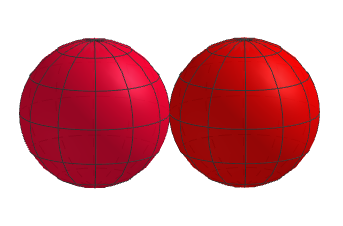
\includegraphics[scale=0.5]{images/S2VS2}
	\end{center}
	\item<4-> $\beta_2 = 2$
	\item<5-> What are $\beta_0$ and $\beta_1$?
	\item<6-> $\beta_0 = 1$ and $\beta_1 = 0$.
	\end{itemize}
\end{itemize}
\end{frame}
%---------------------------------------------------------
